%------------------------------------------------------------------------
% Presentation example for students by Markus Koschi
%
% compile with LaTeX + dvips + ps2pdf or 
% compile with PdfLaTeX after removing all eps figures 

\pdfminorversion=7

%------------------------------------------------------------------------
\documentclass[shortpres,aspectratio=43]{beamer}
%\documentclass[shortpres,aspectratio=169]{beamer}
\usetheme{CambridgeUS}

\setbeamertemplate{footline}
{
  \leavevmode%
  \hbox{%
  \begin{beamercolorbox}[wd=.333333\paperwidth,ht=2.25ex,dp=1ex,left]{author in head/foot}%
  \hspace*{4ex}\usebeamerfont{author in head/foot}\insertshortauthor%~~\beamer@ifempty{\insertshortinstitute}{}{(\insertshortinstitute)}
  \end{beamercolorbox}%
  \begin{beamercolorbox}[wd=.333333\paperwidth,ht=2.25ex,dp=1ex,center]{title in head/foot}%
    \usebeamerfont{title in head/foot}\insertshorttitle
  \end{beamercolorbox}%
  \begin{beamercolorbox}[wd=.333333\paperwidth,ht=2.25ex,dp=1ex,right]{date in head/foot}%
    %\usebeamerfont{date in head/foot}\insertshortdate{}\hspace*{2em}
    \insertframenumber{} / \inserttotalframenumber\hspace*{2ex}
  \end{beamercolorbox}}%
  \vskip0pt%
}\part{title}
\beamertemplatenavigationsymbolsempty

%color specification-----------------------------------------------------
\definecolor{TUMblue}{RGB}{27, 94, 170}%{rgb}{0.00, 0.40, 0.74}
\definecolor{TUMgray}{rgb}{0.85, 0.85, 0.86}
\definecolor{TUMpantone285C}{rgb}{0.00, 0.45, 0.81}
\definecolor{TUMpantone300C}{RGB}{27, 94, 170} %uncorrected TUMpantone300C
\definecolor{lightblue}{RGB}{213,227,241}%{rgb}{0.7529,0.8118,0.9333}

\setbeamercolor{block title}{fg=white, bg=TUMblue}
\setbeamercolor{block body}{bg=lightblue}
\setbeamertemplate{blocks}[rounded][shadow=true]

%------------------------------------------------------------------------
\setbeamercolor{frametitle}{bg=TUMblue, fg=white}
\setbeamercolor{palette primary}{bg=TUMblue, fg=white}%{fg=TUMblue,bg=TUMgray}
\setbeamercolor{palette secondary}{use=palette primary,bg=TUMblue, fg=white}
\setbeamercolor{palette tertiary}{use=palette primary,fg=white, bg=TUMblue}
\setbeamercolor{palette quaternary}{use=palette primary,fg=white, bg=TUMblue}

\setbeamercolor{title}{bg=TUMblue,fg=white}
\setbeamercolor{item projected}{use=item,fg=black,bg = lightblue}
\setbeamercolor{block title}{fg=black, bg=lightblue}
\setbeamercolor{block body}{bg=white}
\setbeamertemplate{blocks}[rounded][shadow=true]

%------------------------------------------------------------------------
\setbeamertemplate{bibliography item}{\insertbiblabel}
\setbeamercolor{bibliography item}{parent=palette primary}
\setbeamercolor{bibliography entry author}{fg=TUMblue}

% define vspace size 
\newlength{\mylength}
\setlength{\mylength}{0.1cm}

%------------------------------------------------------------------------
\usepackage{subfigure}
\usepackage{textpos} % for figure (logo) on slides
\usepackage{psfrag} % for \psfrag in figures
%\usepackage{algorithm,algpseudocode} % for algorithm environment
%\usepackage{booktabs} % for rulers in tables
\usepackage{units} % for units to values
%\usepackage{hyperref}
%\usepackage{graphicx}
\usepackage{tikz}
\usepackage{color}
\usepackage{mathtools}
\usepackage{amsmath}
\usepackage{amsfonts}
\usepackage{svg}
\usepackage{tikz}
\usepackage{pgfplots}

%-----------------------------------------------------------------------
\newcommand{\at}{\fontfamily{ptm}\selectfont @}
\newcommand{\ra}[1]{\renewcommand{\arraystretch}{#1}} %to change the row spacing in tables

\newcommand\blfootnote[1]{%
  \begingroup
  \renewcommand\thefootnote{}\footnote{#1}%
  \addtocounter{footnote}{-1}%
  \endgroup
}

%-----------------------------------------------------------------------
\title[Title]{eBPF-Assisted Relays for Multimedia Streaming}

\author[Name]{Daniel Alexander Antonius Pfeifer}
\institute[TU M\"unchen]{Technical University of Munich}

\date\today

%---------------------------------------------------------------------
\begin{document}

%% TUM logo
\addtobeamertemplate{frametitle}{}{%
\begin{textblock*}{\textwidth}(.91\textwidth,-0.925cm) % for aspectratio=43

\includegraphics[height=0.65cm]{./figures/TUM_Logo_weiss_e.eps} % for aspectratio=43
%\begin{textblock*}{\textwidth}(.92\textwidth,-0.93cm) % for aspectratio=169
%
\includegraphics[height=0.7cm]{./figures/TUM_Logo_weiss_e.eps} % for aspectratio=169
\end{textblock*}}


\begin{frame}[plain]
    \titlepage%
\end{frame}

\begin{frame}{}
  \tableofcontents
\end{frame}


% Interesting figures:
\iffalse%
figures/02_background/adaptive-bitrate-streaming.drawio.pdf
figures/02_background/general-relay.drawio.pdf
figures/02_background/hook-point-locations.drawio.pdf

figures/03_fast_relays/forward-registration.drawio.pdf (maybe too detailed)
figures/03_fast_relays/packet-forwarding.drawio.pdf
figures/03_fast_relays/priority-streams.drawio.pdf
figures/03_fast_relays/retransmission.drawio.pdf (maybe too detailed)
figures/03_fast_relays/route-layering.drawio.pdf

figures/04_testing_and_results/delays_small_packets_simple_userspace.pdf
figures/04_testing_and_results/cpu_usage_server_ns.pdf
figures/04_testing_and_results/cpu_usage_relay_ns.pdf
figures/04_testing_and_results/cpu_usage_client_ns.pdf
\fi

% ----------------------------------------------------------------------- Begin Section Introduction 

\section{Introduction}

\begin{frame}{}
  \tableofcontents[currentsection]
\end{frame}

\begin{frame}{Motivation}
    \begin{minipage}{0.3\textwidth}
        \begin{itemize}
            \item Shorten Critical Path
            \vspace{\mylength}
            \item Avoid Network Stack Traversal
            \vspace{\mylength}
            \item Reduce Forwarding Delay
        \end{itemize}
    \end{minipage}\hfill
    \begin{minipage}{0.6\textwidth}
        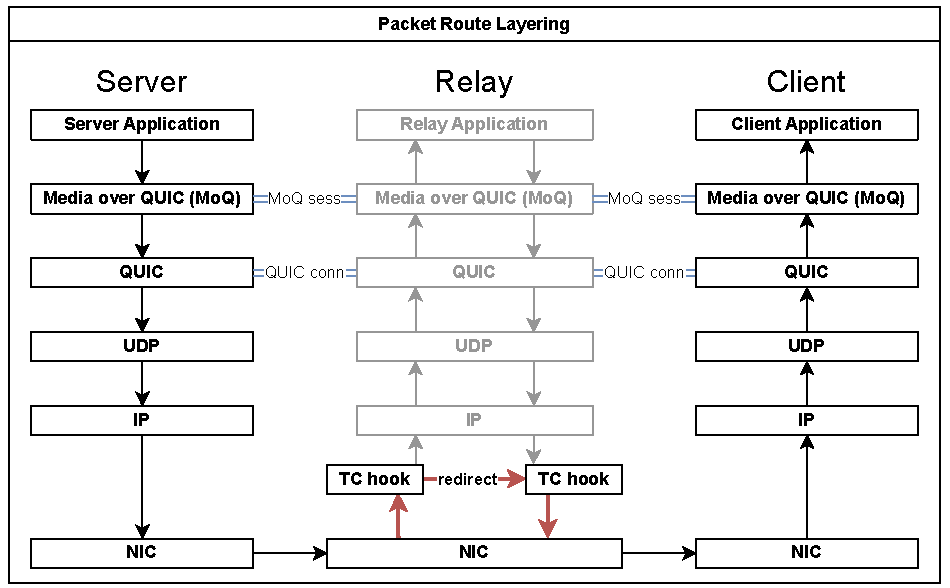
\includegraphics[
            scale=0.45
        ]{../figures/03_fast_relays/route-layering.drawio.pdf}
    \end{minipage}
\end{frame}

\begin{frame}{Research Question}
    \begin{itemize}
        \item \textit{Improve relay performance by using eBPF technology?}
        \vspace{2\mylength}
        \begin{itemize}
            \item \textit{Remove userspace packet-processing from critical path?}
            \vspace{2\mylength}
            \item \textit{Handle packet en- and decryption?}
            \vspace{2\mylength}
            \item \textit{Communication between userspace and the eBPF program?}
            \vspace{2\mylength}
            \item \textit{Generalize to support other protocols?}
        \end{itemize}
    \end{itemize}
\end{frame}

% ----------------------------------------------------------------------- Begin Section QUIC and eBPF

\section{QUIC and eBPF}

\begin{frame}{}
  \tableofcontents[currentsection]
\end{frame}

\begin{frame}{QUIC}
\end{frame}

\begin{frame}{eBPF}
\end{frame}

% ----------------------------------------------------------------------- Begin Section Fast-Relays

\section{Fast-Relays}

\begin{frame}{}
  \tableofcontents[currentsection]
\end{frame}

\begin{frame}{QUIC Adaptations}
\end{frame}

\begin{frame}{eBPF Setup}
\end{frame}

\begin{frame}{Userspace Synchonization}
\end{frame}

\begin{frame}{Congestion Considerations}
\end{frame}

% ----------------------------------------------------------------------- Begin Section Testing

\section{Testing Results}

\begin{frame}{}
  \tableofcontents[currentsection]
\end{frame}

\begin{frame}{Test Setup}
\end{frame}

\begin{frame}{Test Results}
\end{frame}

% ----------------------------------------------------------------------- Begin Section Conclusion and Future Work

\section{Conclusion and Future Work}

\begin{frame}{}
  \tableofcontents[currentsection]
\end{frame}

\begin{frame}{Conclusion}
\end{frame}

\begin{frame}{Future Work}
\end{frame}

\end{document}